\documentclass[%
a4paper,
%twoside,
11pt
]{article}

% encoding, font, language
\usepackage[utf8]{inputenc}
\usepackage[T1]{fontenc}
\usepackage[ngerman, english]{babel}


\usepackage[
    handwritten,
    nowarnings,
    %myconfig
]
{xcookybooky}


\begin{document}

\title{Architecture logicielle \\ Feuille 1}
\author{Benoit Barthes - Anne-laure Mesure}
\maketitle

\section*{Exercice 1}
Avant tout, un bon code est un code qui fonctionne.
Un bon code est un code possédant une architecture claire autant au niveau de l'organisation es fichiers que de la structuration du code en lui-même. On doit avoir un découpage fonctionnel, chaque classe doit avoir un rôle spécifique. Il doit pouvoir être réutilisable et pour ça avoir un couplage faible.
Un bon code est un code compréhensible par tous. Il doit être commenté quand c'est nécessaire et respecter une convention de nommage.
Enfin un bon code est code testé et testable.

\section*{Exercice 2}
\subsection*{1.}
Cette application permet le calcul et l'affichage des factures de clients d'un video club.
\newpage

\subsection*{2.}
\begin{figure}[!ht]
    \center
    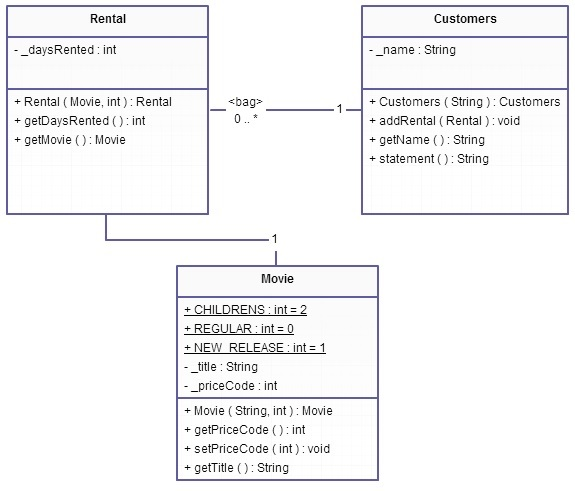
\includegraphics[]{imgs/F1EX2-2.jpg}
    \caption{Diagramme UML avant refactoring}
    %\label{bloghiko}
\end{figure}

\subsection*{3.}
Le principal problème de ce code vient de la méthode statement de la classe Customers, qui fait trop de choses et n'a pas un but précis. Alors qu'elle ne devrait uniquement être responsable de l'affichage, elle calcule également le coût de la location et du total de points de fidélité gagné par le client.\\ A côté de cela, on peut noter le manque d'indentations, de séparation entre les méthodes ainsi que des erreurs de typographie (CHILDRENS au lieu de CHILDREN). La classe Customers   représente un client et ne devrait donc pas être au pluriel.

\section*{Exercice 3}

Dans l'organisation de notre code nous avons créé trois packages, le premier avec le code d'origine, le second avec le code en cours de refactorisation et enfin le troisième avec l'ensemble de nos tests. Nous pouvons ainsi comparer les résultats entre les différents packages et vérifier à chaque évolution que nous ne perdons pas la validité du résultat.

\section*{Exercice 4}

Nous avons donc éclaté progressivement la classe statement en cinq méthodes. Dans un premier temps, nous avons extrait la gestion du prix de la location ainsi que la gestion des points de fidélité. Ce que nous avons noté par la suite est que la responsabilité du calcul du prix d'un film ainsi que des points de fidélités ne revenait pas au client. Tout ce dont on a besoin c'est du film et du nombre de jours de la location, or ces deux informations sont disponibles dans la classe Rental. Nous avons donc extrait le calcul de la location d'un film et l'avons déplacé dans la classe Rental, de même pour le calcul des points de fidélité d'un film.


\section*{Exercice 5}


\section*{Exercice 6}
\section*{Exercice 7}


\end{document} 